\label{sec:overview}

\begin{figure}[!t]
\begin{center}
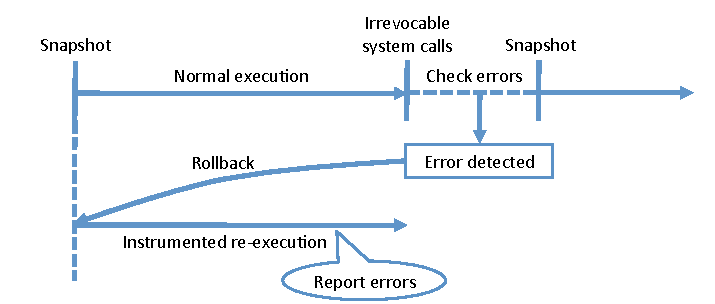
\includegraphics[width=3.3in]{doubletake/figure/overview}
\end{center}
\caption{
Overview of \doubletake{}: execution is divided into epochs at the boundary of irrevocable system calls. 
\label{fig:overview}}
\end{figure}

\doubletake{} aims to reduce the performance overhead of dynamic analyses for memory errors sharing the monotonicity: the evidence of an error is persistent and can be detected after-the-fact. As described in Figure~\ref{fig:overview}, the execution of a program is divided into epochs at irrevocable system calls, discussed in Section~\ref{sec:normal_execution}. Inside each epoch, \doubletake{} allows a program to run at full speed, with the support of checkpointing and very minimum recording overhead. \doubletake{} only checks for evidence of an error when an epoch ends. If an error is detected, \doubletake{} rolls back to the most recent checkpoint and re-execute the program to pinpoint the error.  During the re-execution phase, \doubletake{} can use higher-overhead mechanisms to pinpoint the exact cause of the error. 

Based on this framework, we have implemented three detection tools for heap buffer overflows, use-after-free errors, and memory leaks, which are described in detail in Section~\ref{sec:applications}. 

\doubletake{} employs the following core mechanisms:

\paragraph{Efficient Recording.}
At the beginning of every epoch, \doubletake{} saves a snapshot of program registers, and all writable memory. The epoch ends when the program attempts to issue an irrevocable system call, which is described in Section~\ref{} \CC{here}. \doubletake{} also records the order of thread synchronization operations to support re-execution of parallel programs. \doubletake{} records minimal system state at the beginning of each epoch (like file offsets), which allows system calls that modify this state to be undone if re-execution is required. As a result, most programs require very few epochs and program state checks. We describe the details of each application's state checks in Section~\ref{sec:applications}.

\paragraph{Precise Replay.}
During re-execution, \doubletake{} ensures that all observable system state, system call results, and memory allocations will be the same from the original run. System calls that cannot be replayed, called irrevocable system calls, must be issued at the end of an epoch after detection tools have verified that no errors have occurred. Actually, those system calls consists of the boundary of epochs, which are discussed in Section~\ref{sec:normal_execution}. In practice, most system calls can easily be replayed by handling appropriately. This ensure that most programs run very few integrity checks, and overhead remains low when errors are not detected.

\paragraph{Custom Heap Allocator.}

\doubletake{} replaces the default heap allocator with a BiBOP-style memory allocator, built on HeapLayers~\cite{heaplayers}. \DoubleTake{} pre-allocates a fixed size of memory from its underlying operating system using \texttt{mmap} system calls and satisfies memory allocations from this block by interposing all memory allocation and deallocations. Using the custom memory allocators avoids a big number of sbrk() or mmap() system calls caused by the default memory allocator. In the heap, all heap objects have the block size of {\it power of $2$}, using an object header to mark its status and size information. There is no split and merge operation on heap objects. If the size of an allocation is less than {\it power of 2}, \DoubleTake{} allocates an object with the size of next {\it power of 2}. 




